\documentclass{beamer}
\usetheme{tokitex}

\usepackage{tikz}
\usepackage{graphics}
\usepackage{multirow}
\usepackage{tabto}
\usepackage{xspace}
\usepackage{amsmath}
\usepackage{hyperref}
\usepackage{wrapfig}
\usepackage{mathtools}

\usepackage{tikz}
\usepackage{clrscode3e}
\usepackage{gensymb}

\usepackage[english,bahasa]{babel}
\newtranslation[to=bahasa]{Section}{Bagian}
\newtranslation[to=bahasa]{Subsection}{Subbagian}

\usepackage{listings, lstautogobble}
\usepackage{color}

\definecolor{dkgreen}{rgb}{0,0.6,0}
\definecolor{gray}{rgb}{0.5,0.5,0.5}
\definecolor{mauve}{rgb}{0.58,0,0.82}

\lstset{frame=tb,
  language=c++,
  aboveskip=0mm,
  belowskip=0mm,
  showstringspaces=false,
  columns=fullflexible,
  keepspaces=true,
  basicstyle={\small\ttfamily},
  numbers=none,
  numberstyle=\tiny\color{gray},
  keywordstyle=\color{blue},
  commentstyle=\color{dkgreen},
  stringstyle=\color{mauve},
  breaklines=true,
  breakatwhitespace=true,
  lineskip={-3pt}
}

\usepackage{caption}
\captionsetup[figure]{labelformat=empty}

\newcommand{\progTerm}[1]{\textbf{#1}}
\newcommand{\foreignTerm}[1]{\textit{#1}}
\newcommand{\newTerm}[1]{\alert{\textbf{#1}}}
\newcommand{\emp}[1]{\alert{#1}}
\newcommand{\statement}[1]{"#1"}

\newcommand{\floor}[1]{\lfloor #1 \rfloor}
\newcommand{\ceil}[1]{\lceil #1 \rceil}
\newcommand{\abs}[1]{\left\lvert#1\right\rvert}
\newcommand{\norm}[1]{\left\lVert#1\right\rVert}

% Getting tired of writing \foreignTerm all the time
\newcommand{\farray}{\foreignTerm{array}\xspace}
\newcommand{\fArray}{\foreignTerm{Array}\xspace}
\newcommand{\foverhead}{\foreignTerm{overhead}\xspace}
\newcommand{\fOverhead}{\foreignTerm{Overhead}\xspace}
\newcommand{\fsubarray}{\foreignTerm{subarray}\xspace}
\newcommand{\fSubarray}{\foreignTerm{Subarray}\xspace}
\newcommand{\fbasecase}{\foreignTerm{base case}\xspace}
\newcommand{\fBasecase}{\foreignTerm{Base case}\xspace}
\newcommand{\ftopdown}{\foreignTerm{top-down}\xspace}
\newcommand{\fTopdown}{\foreignTerm{Top-down}\xspace}
\newcommand{\fbottomup}{\foreignTerm{bottom-up}\xspace}
\newcommand{\fBottomup}{\foreignTerm{Bottom-up}\xspace}
\newcommand{\fpruning}{\foreignTerm{pruning}\xspace}
\newcommand{\fPruning}{\foreignTerm{Pruning}\xspace}

\newcommand{\fgraph}{\foreignTerm{graph}\xspace}
\newcommand{\fGraph}{\foreignTerm{Graph}\xspace}
\newcommand{\froot}{\foreignTerm{root}\xspace}
\newcommand{\fRoot}{\foreignTerm{Root}\xspace}
\newcommand{\fnode}{\foreignTerm{node}\xspace}
\newcommand{\fNode}{\foreignTerm{Node}\xspace}
\newcommand{\fedge}{\foreignTerm{edge}\xspace}
\newcommand{\fEdge}{\foreignTerm{Edge}\xspace}
\newcommand{\fcycle}{\foreignTerm{cycle}\xspace}
\newcommand{\fCycle}{\foreignTerm{Cycle}\xspace}
\newcommand{\fdegree}{\foreignTerm{degree}\xspace}
\newcommand{\fDegree}{\foreignTerm{Degree}\xspace}
\newcommand{\fadjacencylist}{\foreignTerm{adjacency list}\xspace}
\newcommand{\fAdjacencylist}{\foreignTerm{Adjacency list}\xspace}
\newcommand{\fadjacencymatrix}{\foreignTerm{adjacency matrix}\xspace}
\newcommand{\fAdjacencymatrix}{\foreignTerm{Adjacency matrix}\xspace}
\newcommand{\fedgelist}{\foreignTerm{edge list}\xspace}
\newcommand{\fEdgelist}{\foreignTerm{Edge list}\xspace}
\newcommand{\flist}{\foreignTerm{list}\xspace}
\newcommand{\fList}{\foreignTerm{List}\xspace}
\newcommand{\fgraphtraversal}{\foreignTerm{graph traversal}\xspace}
\newcommand{\fGraphtraversal}{\foreignTerm{Graph traversal}\xspace}
\newcommand{\ftree}{\foreignTerm{tree}\xspace}
\newcommand{\fTree}{\foreignTerm{Tree}\xspace}
\newcommand{\fsubtree}{\foreignTerm{subtree}\xspace}
\newcommand{\fSubtree}{\foreignTerm{Subtree}\xspace}
\newcommand{\fparent}{\foreignTerm{parent}\xspace}
\newcommand{\fParent}{\foreignTerm{Parent}\xspace}
\newcommand{\fsibling}{\foreignTerm{sibling}\xspace}
\newcommand{\fSibling}{\foreignTerm{Sibling}\xspace}
\newcommand{\fpath}{\foreignTerm{path}\xspace}
\newcommand{\fPath}{\foreignTerm{Path}\xspace}
\newcommand{\fconnectedcomponent}{\foreignTerm{connected component}\xspace}
\newcommand{\fConnectedcomponent}{\foreignTerm{Connected component}\xspace}
\newcommand{\fbridge}{\foreignTerm{bridge}\xspace}
\newcommand{\fBridge}{\foreignTerm{Bridge}\xspace}
\newcommand{\farticulationpoint}{\foreignTerm{articulation point}\xspace}
\newcommand{\fArticulationpoint}{\foreignTerm{Articulation point}\xspace}
\newcommand{\ftreeedge}{\foreignTerm{tree edge}\xspace}
\newcommand{\fTreeedge}{\foreignTerm{Tree edge}\xspace}
\newcommand{\fbackedge}{\foreignTerm{back edge}\xspace}
\newcommand{\fBackedge}{\foreignTerm{Back edge}\xspace}
\newcommand{\fforwardedge}{\foreignTerm{forward edge}\xspace}
\newcommand{\fForwardedge}{\foreignTerm{Forward edge}\xspace}
\newcommand{\fcrossedge}{\foreignTerm{cross edge}\xspace}
\newcommand{\fCrossedge}{\foreignTerm{Cross edge}\xspace}
\newcommand{\fdiscoverytime}{\foreignTerm{discovery time}\xspace}
\newcommand{\fDiscoverytime}{\foreignTerm{Discovery time}\xspace}
\newcommand{\flowlink}{\foreignTerm{low link}\xspace}
\newcommand{\fLowlink}{\foreignTerm{Low link}\xspace}
\newcommand{\fstack}{\foreignTerm{stack}\xspace}
\newcommand{\fStack}{\foreignTerm{Stack}\xspace}
\newcommand{\for}{\foreignTerm{or}\xspace}
\newcommand{\fOr}{\foreignTerm{Or}\xspace}
\newcommand{\fand}{\foreignTerm{and}\xspace}
\newcommand{\fAnd}{\foreignTerm{And}\xspace}
\newcommand{\fcentroid}{\foreignTerm{centroid}\xspace}
\newcommand{\fCentroid}{\foreignTerm{Centroid}\xspace}

\newcommand{\fDivideAndConquer}{\foreignTerm{Divide and conquer}\xspace}
\newcommand{\fdivideAndConquer}{\foreignTerm{divide and conquer}\xspace}
\newcommand{\fMergeSort}{\foreignTerm{Merge sort}\xspace}
\newcommand{\fmergeSort}{\foreignTerm{merge sort}\xspace}
\newcommand{\fQuickSort}{\foreignTerm{Quicksort}\xspace}
\newcommand{\fquickSort}{\foreignTerm{quicksort}\xspace}
\newcommand{\fpivot}{\foreignTerm{pivot}\xspace}
\newcommand{\fPivot}{\foreignTerm{Pivot}\xspace}
\newcommand{\fbruteForce}{\foreignTerm{brute force}\xspace}
\newcommand{\fBruteForce}{\foreignTerm{Brute force}\xspace}
\newcommand{\fCompleteSearch}{\foreignTerm{complete search}\xspace}
\newcommand{\fExhaustiveSearch}{\foreignTerm{exhaustive search}\xspace}
\newcommand{\fbinarySearch}{\foreignTerm{binary search}\xspace}
\newcommand{\fBinarySearch}{\foreignTerm{Binary search}\xspace}
\newcommand{\fternarySearch}{\foreignTerm{ternary search}\xspace}
\newcommand{\fTernarySearch}{\foreignTerm{Ternary search}\xspace}
\newcommand{\funimodal}{\foreignTerm{unimodal}\xspace}
\newcommand{\fUnimodal}{\foreignTerm{Unimodal}\xspace}
\newcommand{\fGreedy}{\foreignTerm{Greedy}\xspace}
\newcommand{\fgreedy}{\foreignTerm{greedy}\xspace}
\newcommand{\fgreedyChoice}{\foreignTerm{greedy choice}\xspace}
\newcommand{\fGreedyChoice}{\foreignTerm{Greedy choice}\xspace}

\newcommand{\fdp}{\foreignTerm{dynamic programming}\xspace}
\newcommand{\fDp}{\foreignTerm{Dynamic programming}\xspace}
\newcommand{\fbitmask}{\foreignTerm{bitmask}\xspace}
\newcommand{\fBitmask}{\foreignTerm{Bitmask}\xspace}
\newcommand{\fstate}{\foreignTerm{state}\xspace}
\newcommand{\fState}{\foreignTerm{State}\xspace}
\newcommand{\fsubmask}{\foreignTerm{submask}\xspace}
\newcommand{\fSubmask}{\foreignTerm{Submask}\xspace}

\newcommand{\pheap}{\foreignTerm{heap}\xspace}
\newcommand{\pHeap}{\foreignTerm{Heap}\xspace}
\newcommand{\pBinaryHeap}{\foreignTerm{Binary Heap}\xspace}
\newcommand{\pbinaryHeap}{\foreignTerm{binary heap}\xspace}
\newcommand{\pHeapsort}{\foreignTerm{Heapsort}\xspace}
\newcommand{\pheapsort}{\foreignTerm{heapsort}\xspace}
\newcommand{\pdjs}{\foreignTerm{disjoint set}\xspace}
\newcommand{\pDjs}{\foreignTerm{Disjoint set}\xspace}

\newcommand{\fdotProduct}{\foreignTerm{dot product}\xspace}
\newcommand{\fDotProduct}{\foreignTerm{Dot product}\xspace}
\newcommand{\fcrossProduct}{\foreignTerm{cross product}\xspace}
\newcommand{\fCrossProduct}{\foreignTerm{Cross product}\xspace}
\newcommand{\fconvexHull}{\foreignTerm{convex hull}\xspace}
\newcommand{\fConvexHull}{\foreignTerm{Convex hull}\xspace}
\newcommand{\fgrahamScan}{\foreignTerm{graham scan}\xspace}
\newcommand{\fGrahamScan}{\foreignTerm{Graham scan}\xspace}
\newcommand{\flineSweep}{\foreignTerm{line sweep}\xspace}
\newcommand{\fLineSweep}{\foreignTerm{Line sweep}\xspace}

\newcommand{\fset}{\foreignTerm{set}\xspace}
\newcommand{\fSet}{\foreignTerm{Set}\xspace}
\newcommand{\fprefixSum}{\foreignTerm{prefix sum}\xspace}
\newcommand{\fPrefixSum}{\foreignTerm{Prefix sum}\xspace}
\newcommand{\ffenwickTree}{\foreignTerm{fenwick tree}\xspace}
\newcommand{\fFenwickTree}{\foreignTerm{Fenwick tree}\xspace}
\newcommand{\frangeSumQuery}{\foreignTerm{range sum query}\xspace}
\newcommand{\fRangeSumQuery}{\foreignTerm{Range sum query}\xspace}
\newcommand{\fquery}{\foreignTerm{query}\xspace}
\newcommand{\fQuery}{\foreignTerm{Query}\xspace}
\newcommand{\fsegmentTree}{\foreignTerm{segment tree}\xspace}
\newcommand{\fSegmentTree}{\foreignTerm{Segment tree}\xspace}
\newcommand{\fbinaryTree}{\foreignTerm{binary tree}\xspace}
\newcommand{\fBinaryTree}{\foreignTerm{Binary tree}\xspace}
\newcommand{\flazyPropagation}{\foreignTerm{lazy propagation}\xspace}
\newcommand{\fLazyPropagation}{\foreignTerm{Lazy propagation}\xspace}
\newcommand{\fsparseTable}{\foreignTerm{sparse table}\xspace}
\newcommand{\fSparseTable}{\foreignTerm{Sparse table}\xspace}

\newcommand{\ftrail}{\foreignTerm{trail}\xspace}
\newcommand{\fTrail}{\foreignTerm{Trail}\xspace}
\newcommand{\feulerTour}{\foreignTerm{euler tour}\xspace}
\newcommand{\fEulerTour}{\foreignTerm{Euler tour}\xspace}
\newcommand{\feulerTourTree}{\foreignTerm{euler tour tree}\xspace}
\newcommand{\fEulerTourTree}{\foreignTerm{Euler tour tree}\xspace}

\newcommand{\fmaxflow}{\foreignTerm{maximum flow}\xspace}
\newcommand{\fMaxflow}{\foreignTerm{Maximum flow}\xspace}
\newcommand{\fmincut}{\foreignTerm{minimum cut}\xspace}
\newcommand{\fMincut}{\foreignTerm{Minimum cut}\xspace}
\newcommand{\fflow}{\foreignTerm{flow}\xspace}
\newcommand{\fFlow}{\foreignTerm{Flow}\xspace}
\newcommand{\fsource}{\foreignTerm{source}\xspace}
\newcommand{\fSource}{\foreignTerm{Source}\xspace}
\newcommand{\fsink}{\foreignTerm{sink}\xspace}
\newcommand{\fSink}{\foreignTerm{Sink}\xspace}
\newcommand{\fbackEdge}{\foreignTerm{back-edge}\xspace}
\newcommand{\fBackEdge}{\foreignTerm{Back-edge}\xspace}
\newcommand{\fresidualCapacity}{\foreignTerm{residual capacity}\xspace}
\newcommand{\fResidualCapacity}{\foreignTerm{Residual capacity}\xspace}
\newcommand{\fbottleneck}{\foreignTerm{bottleneck}\xspace}
\newcommand{\fBottleneck}{\foreignTerm{Bottleneck}\xspace}
\newcommand{\faugmentingPath}{\foreignTerm{augmenting path}\xspace}
\newcommand{\fAugmentingPath}{\foreignTerm{Augmenting path}\xspace}


\title{Dasar-Dasar Geometri}
\author{Tim Olimpiade Komputer Indonesia}
\date{}

\begin{document}

\begin{frame}
\titlepage
\end{frame}

\begin{frame}
\frametitle{Pendahuluan}
Melalui dokumen ini, kalian akan:
\begin{itemize}
  \item Mengetahui dasar-dasar geometri yang digunakan pada kompetisi pemrograman.
  \item Mengingat kembali definisi-definisi matematis elemen geometri.
\end{itemize}
\end{frame}

\begin{frame}
\frametitle{Titik}
\begin{itemize}
  \item \newTerm{Titik} merupakan elemen mendasar pada dunia geometri.
  \item Titik dapat didefinisikan pada 2 dimensi, 3 dimensi, atau lebih.
  \item Pada persoalan pemrograman, umumnya titik didefinisikan pada bidang 2 dimensi.
  \item Pada bidang 2 dimensi, titik dapat dianggap berada pada suatu koordinat ($x$, $y$).
  \item Representasi titik pada program dapat diwujudkan dengan kelompok data yang menyimpan nilai $x$ dan $y$.
  \item Kelompok data ini misalnya \progTerm{record} (Pascal), \progTerm{struct} (C) atau \progTerm{class} (C++/Java).
\end{itemize}
\end{frame}

\begin{frame}
\frametitle{Garis}
\begin{itemize}
  \item \newTerm{Garis} merupakan himpunan seluruh titik ($x$, $y$), yang memenuhi suatu persamaan $Ax + By = C$, dengan $A, B,$ dan $C$ merupakan suatu bilangan riil.
  \item Bentuk lain dari persamaan garis yang umum adalah $y = mx + c$, dengan $m$ dan $c$ suatu bilangan riil.
\end{itemize}  
\begin{figure}
  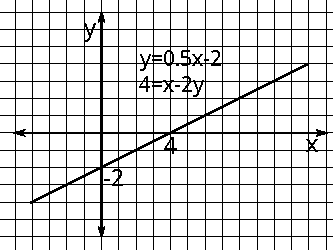
\includegraphics[width=6cm]{asset/line.pdf}
\end{figure}
\end{frame}

\begin{frame}
\frametitle{Garis (lanj.)}
\begin{itemize}
  \item Untuk merepresentasikan garis, kita dapat membuat kelompok data yang menyimpan nilai $<A, B, C>$, atau $<m, c>$, bergantung pada persamaan yang Anda gunakan. 
  \item Apabila ditelusuri, kedua persamaan ini sebenarnya berkaitan:
\begin{eqnarray*}
Ax + By &=& C \\
By &=& C - Ax \\
y &=& \frac{C}{B} - \frac{A}{B}x \\
y &=& \left(-\frac{A}{B}\right)x + \frac{C}{B} 
\end{eqnarray*}
  \item Jadi $m = -\frac{A}{B}$ dan $c = \frac{C}{B}$.
\end{itemize}
\end{frame}

\begin{frame}
\frametitle{Garis Vertikal }
\begin{itemize}
  \item Hati-hati saat merepresentasikan garis vertikal, misalnya $x = 3$.
  \item Representasi $Ax + By = C$ dapat merepresentasikannya, yaitu dengan $A=1, B=0, C=3$.
\end{itemize}
\begin{figure}
  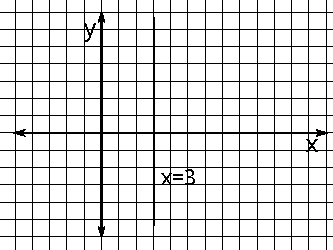
\includegraphics[width=6cm]{asset/vertical-line.pdf}
\end{figure}
\end{frame}

\begin{frame}
\frametitle{Garis Vertikal (lanj.)}
\begin{itemize}
  \item Sementara representasi $y = mx + c$ memiliki kesulitan, karena nilai $m$ yang tidak terdefinisi:
\begin{eqnarray*}
m &=& -\frac{A}{B} \\
&=& -\frac{1}{0}
\end{eqnarray*}
  \item Untuk kasus yang mungkin terdapat garis vertikal, representasi $Ax + By = C$ lebih disarankan.
\end{itemize}
\end{frame}


\begin{frame}
\frametitle{Segmen Garis}
\begin{itemize}
  \item \newTerm{Segmen garis} merupakan garis yang terdefinisi dari suatu titik $(x_1, y_1)$ ke titik $(x_2, y_2)$
  \item Perhatikan bahwa berbeda dengan segmen garis, garis memiliki panjang yang tak berhingga.
  \item Segmen garis dapat direpresentasikan dengan dua titik, yaitu ujung-ujungnya.
\end{itemize}
\begin{figure}
  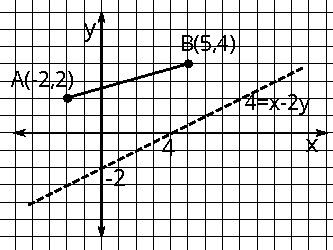
\includegraphics[width=6cm]{asset/line-vs-line-segment.pdf}
\end{figure}
\end{frame}

\begin{frame}
\frametitle{Jarak Euclidean}
\begin{itemize}
  \item \newTerm{Jarak Euclidean} adalah definisi jarak yang umum digunakan pada bidang 2 dimensi atau ruang 3 dimensi.
  \item Jarak pada bidang 2 dimensi dari dua titik A(x, y) dan B(x, y) adalah:

  \(dist(A, B) = \sqrt{(A.x - B.x)^2 + (A.y - B.y)^2} \)
  \item Anda dapat menggunakan rumus ini untuk mengetahui panjang dari segmen garis.
\end{itemize}
\begin{figure}
  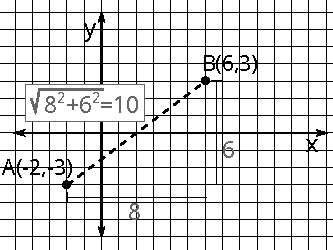
\includegraphics[width=6cm]{asset/euclidean.pdf}
\end{figure}
\end{frame}

\begin{frame}
\frametitle{Segitiga}
\begin{itemize}
  \item \newTerm{Segitiga} merupakan bangun 2 dimensi yang paling mendasar.
  \item Segitiga terdiri dari 3 titik sudut, yang mana antar titik sudut terhubung oleh segmen garis.
  \item Berdasarkan panjang segmen garisnya, segitiga dapat berupa segitiga sama kaki, sama sisi, siku-siku, atau sembarang.
\end{itemize}
\begin{figure}
  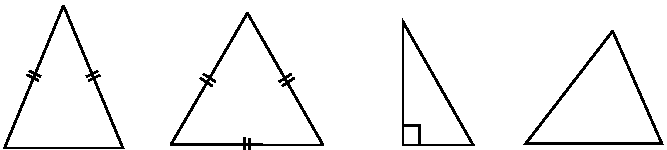
\includegraphics[width=6cm]{asset/triangles.pdf}
\end{figure}
\end{frame}

\begin{frame}
\frametitle{Teorema Pythagoras}
\begin{itemize}
  \item Pada segitiga siku-siku, kita dapat mengetahui panjang sisi miringnya menggunakan rumus Teorema Pythagoras.
  
  \(a^2 + b^2 = c^2\)
\end{itemize}
\begin{figure}
  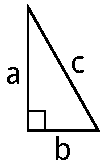
\includegraphics[width=1.5cm]{asset/pythagoras.pdf}
\end{figure}
\end{frame}

\begin{frame}
\frametitle{Luas Segitiga}
\begin{itemize}
  \item Rumus klasik dari luas segitiga dengan panjang alas $a$ dan tinggi $t$ adalah:\newline
  
  \(\displaystyle L = \frac{a \times t}{2}\)
\end{itemize}
\begin{figure}
  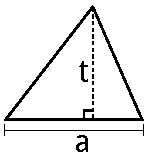
\includegraphics[width=3cm]{asset/triangle-area.pdf}
\end{figure}
\end{frame}

\begin{frame}
\frametitle{Luas Segitiga (Rumus Heron)}
\begin{itemize}
  \item Ada kalanya kita tidak tahu tinggi dari segitiga, sehingga rumus sebelumnya tidak dapat digunakan.
  \item Alternatif lain adalah menggunakan \newTerm{rumus Heron}, yaitu:\newline
    
  \(\displaystyle L = \sqrt{s(s-a)(s-b)(s-c)} \) \newline 
  
  dengan \(\displaystyle s = \frac{a+b+c}{2}\)
  
\end{itemize}
\begin{figure}
  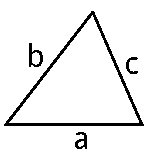
\includegraphics[width=2.5cm]{asset/triangle-heron.pdf}
\end{figure}
\end{frame}

\begin{frame}
\frametitle{Sudut Segitiga}
\begin{itemize}
  \item Jumlah sudut-sudut pada suatu segitiga adalah $180^{\circ}$.
\end{itemize}
\begin{figure}
  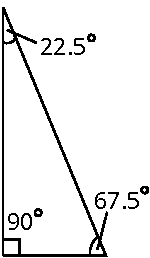
\includegraphics[width=2.5cm]{asset/triangle-angle.pdf}
\end{figure}
\end{frame}

\begin{frame}
\frametitle{Segi-N}
\begin{itemize}
  \item Untuk segi-$N$, jumlah sudut-sudutnya adalah $180(N - 2)^{\circ}$.
  \item Misalnya untuk segi-4, jumlah sudut-sudutnya adalah $180(4 - 2)^{\circ} = 360^{\circ}$
\end{itemize}
\begin{figure}
  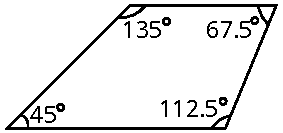
\includegraphics[width=5cm]{asset/quadrangle-angle.pdf}
\end{figure}
\end{frame}

\begin{frame}
\frametitle{Lingkaran}
\begin{itemize}
  \item Lingkaran dengan titik pusat $(x_p, y_p)$ dan jari-jari $r$ merupakan himpunan seluruh titik $(x, y)$ yang memenuhi $(x - x_p)^2 + (y - y_p)^2 = r^2$.
\end{itemize}
\begin{figure}
  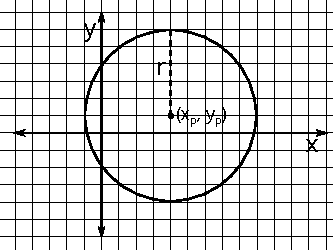
\includegraphics[width=6cm]{asset/circle.pdf}
\end{figure}
\end{frame}

\begin{frame}
\frametitle{Properti Lingkaran}
\begin{itemize}
  \item Luas dari lingkaran dengan jari-jari $r$ adalah $\pi r^2$.
  \item Keliling dari lingkaran dengan jari-jari $r$ adalah $2\pi r$.
  \item Diameter lingkaran merupakan dua kali jari-jari, atau $2r$.
\end{itemize}
\end{frame}

\begin{frame}
\frametitle{Tentang Pi}
\begin{itemize}
  \item Pi merupakan konstanta dalam matematika, dan digunakan dalam pencarian luas atau keliling lingkaran.
  \item Hati-hati! Nilai pi \textbf{tidak sama dengan} \(\displaystyle \frac{22}{7}\).
  \item Penggunaan \(\displaystyle \frac{22}{7}\) hanyalah aproksimasi dari nilai pi yang sesungguhnya.
\end{itemize}
\begin{eqnarray*}
\pi &=& 3.14159265359.. \\
\\
\frac{22}{7} &=& 3.14285714285..
\end{eqnarray*}
\end{frame}

\begin{frame}
\frametitle{Tentang Pi (lanj.)}
\begin{itemize}
  \item Untuk perhitungan pada kompetisi pemrograman, Anda dapat menggunakan nilai pi yang diberikan pada soal.
  \item Jika soal tidak memberikan nilai pi yang digunakan, Anda dapat mencarinya dengan fungsi \foreignTerm{arc-cosinus}, yaitu fungsi pada trigonometri.
  \item Nilai pi didapatkan dari:
  \begin{itemize}
    \item Pascal: $arccos(-1)$
    \item C++: $acos(-1)$ (memerlukan include cmath)
  \end{itemize}
  \item Trigonometri sendiri tidak termasuk dalam silabus kompetisi pemrograman tingkat SMA, sehingga Anda tidak perlu memperdalamnya.
\end{itemize}
\end{frame}

\begin{frame}
\frametitle{Pesan Tentang Presisi}
\begin{itemize}
  \item Sebisa mungkin, gunakan tipe data bilangan bulat.
  \item Apabila Anda terpaksa menggunakan tipe data bilangan riil, seperti \progTerm{real} atau \progTerm{double}, terapkan kiat-kiat yang telah Anda pelajari pada pemrograman dasar.
  \item Sebagai contoh, untuk membandingkan dua bilangan, periksa apakah selisih absolut dari kedua bilangan lebih kecil dari suatu nilai toleransi, yang biasa disebut \textit{epsilon} ($\epsilon$).
  \begin{codebox}
  \Procname{$\proc{isEqual}(a, b)$}
     \Return $\proc{abs}(a - b) < \epsilon$
  \end{codebox}
  \item Nilai toleransi yang biasa digunakan adalah $10^{-12}$.
\end{itemize}
\end{frame}

\begin{frame}
\frametitle{Penutup}
\begin{itemize}
  \item Komputasi geometri merupakan topik yang sangat luas, dan baru kita bahas sebagian kecil.
  \item Pada kesempatan yang lain, kita akan mempelajari teknik merepresentasikan elemen geometri menggunakan konsep matematika yang lebih kompleks, yaitu vektor.
\end{itemize}
\end{frame}

% NEXT:
%vektor
%dot product
%cross product
%luas segitiga dari 3 titik
%CCW test
%line segment intersection
%line segment intersection getPoint
%poligon
%poligon konveks / non
%poligon area
%titik dalam poligon
%graham's scan
\end{document}
